%!TEX root = ../main.tex
 \section{Mining Background}
Mining is a key part of this thesis, while not an in depth knowledge of mining is required, basic information is needed for problem definitions and clarity of communication. The focus of the thesis is the removal of overburden from strip mines using draglines, as this is a specific topic and not a general discussion on optimisation of mining machines in general only information on draglines and the environment in which they operate should be considered. Mining is a huge industry in Australia, making up 5.6\% of the nations GDP \cite{ExportStats} it is obvious that optimisation and planning is fitting in this field of industry\cite{DraglineDecade}.
However for mathematical models to be developed a thorough understanding of draglines should be gained to ensure the accuracy and validity of all formulated models. 
\subsection{Strip Mining}
Strip mining is the practice of removing a seam of material by removing strips of soil and overburden \cite{IntoOpenPit} to expose the underlying ore, this method is typically only viable near the surface, as a result some of the largest machines in the world are used in strip mining. Two techniques exist for the removal of overburden in strip mining \cite{Workpls} however here only the first will be considered. That is the flattening of an open area removal of overburden through strips. These strips span the length of the mine and will be removed sequentially, with the overburden from the current strip being dumped into emptied strips adjacent\cite{SMEBOOK}. Strip mining will recover a greater percentage of Ore and at a faster rate in comparison to underground methods \cite{SMEBOOK}, and as such is preferable when the appropriate conditions are met. Many machines are used in the process of strip mining, one in this process is the dragline which removes the overburden from a strip exposing the ore below\cite{IntoOpenPit}.
\subsection{Blocks}
A block is an element of  strip in which the dragline moves, these blocks make up a strip in an open cut mine. \cite{SMEBOOK} Draglines will not just move from the beginning of the strip to the end in a straight line, instead they move in patterns within the block \cite{IntoOpenPit}. This pattern is already the object of optimisation as the reduction of time spent within a block will itself reduce the total time taken to remove overburden from a strip. While the movement patterns within a block can vary from block to block it is assumed that they remain the same for this thesis. A block must be mined before all blocks after it. 
\begin{figure}[h]
\caption{Top down block view}
\label{blk}
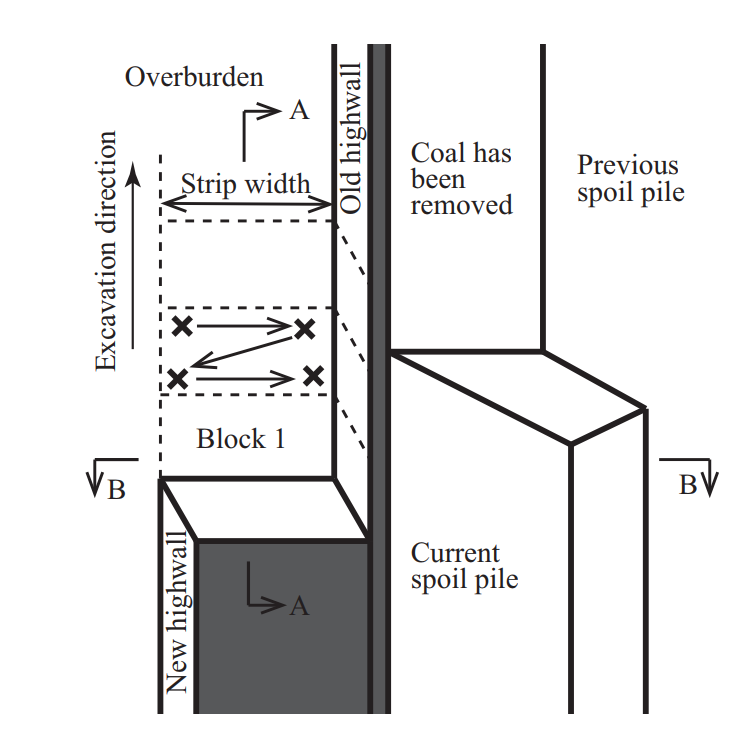
\includegraphics[width=\textwidth]{Block.png}
\end{figure}
\begin{figure}[h]
\caption{Side block view}
\label{blk}
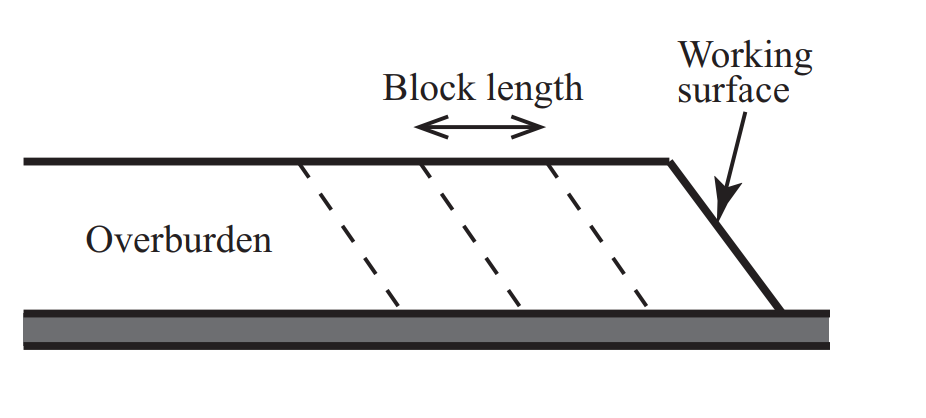
\includegraphics[width=\textwidth]{blockside.png}
\end{figure}

\subsection{Draglines}
A dragline is a massive machine used in open cut mining, working in strips to remove the overburden from a mine to expose the ore below\cite{ORPlanning}. The process that is done to achieve this is simple and cyclical in nature, first the bucked of the dragline is positioned above the material to be removed. Then it is lowered and pulled along the surface of the overburden, once the bucket is full it is lifted and moved above a spoil channel where it is deposited and the cycle is started again \cite{Dynamic Model}. The movement of a dragline may occur on two axis, a rotation or swing and a lift or hoist; these two actions convey the cost associated with using a dragline as they will typically be the only unique motions associated with both overburden removal and spoil dumping\cite{A*Search}. 


\section{Operations Research Background}
The field of operations research is a mathematical discipline specialising in the application of advanced analytical methods to make better decisions for specified problems \cite{Intro2or}. Often considered as a subsection of applied mathematics operations research employs techniques from mathematical modelling and optimization theory to calculate optimal or near optimal solutions to complex decision making problems\cite{abtOR} \\ Naturally this branch of mathematics lends itself to the problem of optimal block dimensions in a strip mine, with the use of optimal decisions through either precise calculation or policy the best possible solution can be found using the field of operations research. The scope of this field is diverse, with many potential solutions to a problem. As such the selection of mathematical modelling and optimisation techniques should be considered carefully to result in an accurate solution. 
\\
Mathematical modelling is a vital section of operations research, however the problem can be written and formulated in many different ways, as such the specific formulation styles of a technique will also be mentioned in that section, modelling in general can follow some simple rules yet no overall method or technique exists for the creation of a mathematical model, it is instead reliant on understanding of the system. 

\subsection{Linear Programming}
Linear programming is a technique used to obtain the optimal outcome of a model such as the minimal time or highest profit\cite{LPII}. This method can only be applied to a mathematical model with a linear objective function subject to linear equality and linear inequality constraints\cite{Intro2or}.\\ Often the model is described as groups of variables and constraints with an overall objective function. This method of optimisation is often solved using complex optimisation engines such as gurobi rather than through algorithms implemented specifically for the implementation. The process of optimisation is done by defining a feasible region of valid solutions as a convex $n^{th}$ dimensional polytope, where $n$ is the dimensionality of the variables associated\cite{oriNTRO}. Here this polytope is defined as an intersection of a finite amount of half spaces defined by linear inequalities. Within this polytope the optimal feasible solution will be found on a vertex satisfying all constraints and the objective function, this method can be calculated using matrix manipulation in algorithms such as the modified simplex algorithm\cite{LP}.  	
\\
The standard variables in a linear program are continuous, however a sub technique of linear programming is integer programming which adds the constraint that some variables must be full positive integers \cite{LPII}. This problem is typically harder to solve as the optimal linear solution may not be similar to the optimal integer solution\cite{Intro2or}. An integer solution is often calculated by calculating an optimal linear solution and branching on rounding decisions \cite{LPII} for the integer variables to create a decision tree. This tree is branched such that the difference between the linear solution and chosen integer solution is minimised, this is the origin of the increased difficulty of integer programming in comparison to linear programming\cite{oriNTRO}. 

\subsection{Dynamic Programming} 
Dynamic programming is a method of optimisation in which a sub-problem is solved and the solution stored \cite{Bellman}, this is done for all sub-problems until the full problem can be constructed from, if a sub-problem has already been solved and stored then it is called from memory instead of through calculation \cite{MITDynamic}. The process of storing sub problems for later use is called memotisation\cite{Bellman} and is vital for use in dynamic programming as dynamic programming often encounters similar sub-problems when working recursively\cite{MITDynamic}. \\

Typically a dynamic program refers to recursively breaking down decisions into steps through a stage \cite{DPfound}. The value of each decision in a stage is a combination of the initial myopic value of the choice as well as the value of all other solutions that occur after this decision is made\cite{DPfound}. This requires that some state in the problem is altered when a decision is made, then the affects of this decision must also be considered for all subsequent choices. This creates and expanding tree of subproblems and is why the method of memotisation is so vital to dynamic programming as often the same sub-problem will be encountered multiple times\cite{Bellman}. 
\subsection{Metahueristics} %Should I mention this if I looked into it but never used it
A metahueristic is a higher level optimisation technique used to find, generate or select a heuristic that may provide a good solution to an optimisation problem\cite{Meta}, typically when working with incomplete information , inaccurate information or limited computational power\cite{Meta}. Unlike Linear programming and dynamic progamming a metahueristic does not garuntee a globally optimal solution , due to metahueristics typically relying on stochastic optimisation to generate solutions. \\
The genetic algorithm is such an example of a metahueristic where candidate solutions are evolved to find a better solution\cite{GA}, this is done by calculating the value of all candidates. After this is complete the more preferable solutions are combined with one another in such a way that a new series of candidate solutions is generated \cite{GA}. This is done iteratively until the change between generations is sufficiently small, at this point either a local optimal or global optimal solution can be found. Typically the genetic algorithm is used for determining a policy for good solutions, rather than linear programming or dynamic programming which will calculate the true optimal solution. 
